
\section{Distributed Cooperation Example\marginnote{(Demonstration of synchronizing planning states to coordinate vehicle/task assignments)}}

Given a set of Unmanned Air Vehicles (UAVs) and a set of tasks, planning trajectories and assigning UAVs to perform tasks is a difficult problem. If a Ground Control Station (GCS) is able to communicate to all of the UAVs (\textit{fully connected}),  then the trajectory/assignment problem can be solved \textit{centrally} and the resulting assignment plans can be sent to the UAVs for execution. However, there are scenarios where complete communication channels do not exist and it is desirable to have a team of UAVs that can decide on trajectory/assignments (\textit{cooperate}) by communicating with each other in an ad-hoc/distributed manner. 


\begin{marginfigure}
	\hspace{-35pt}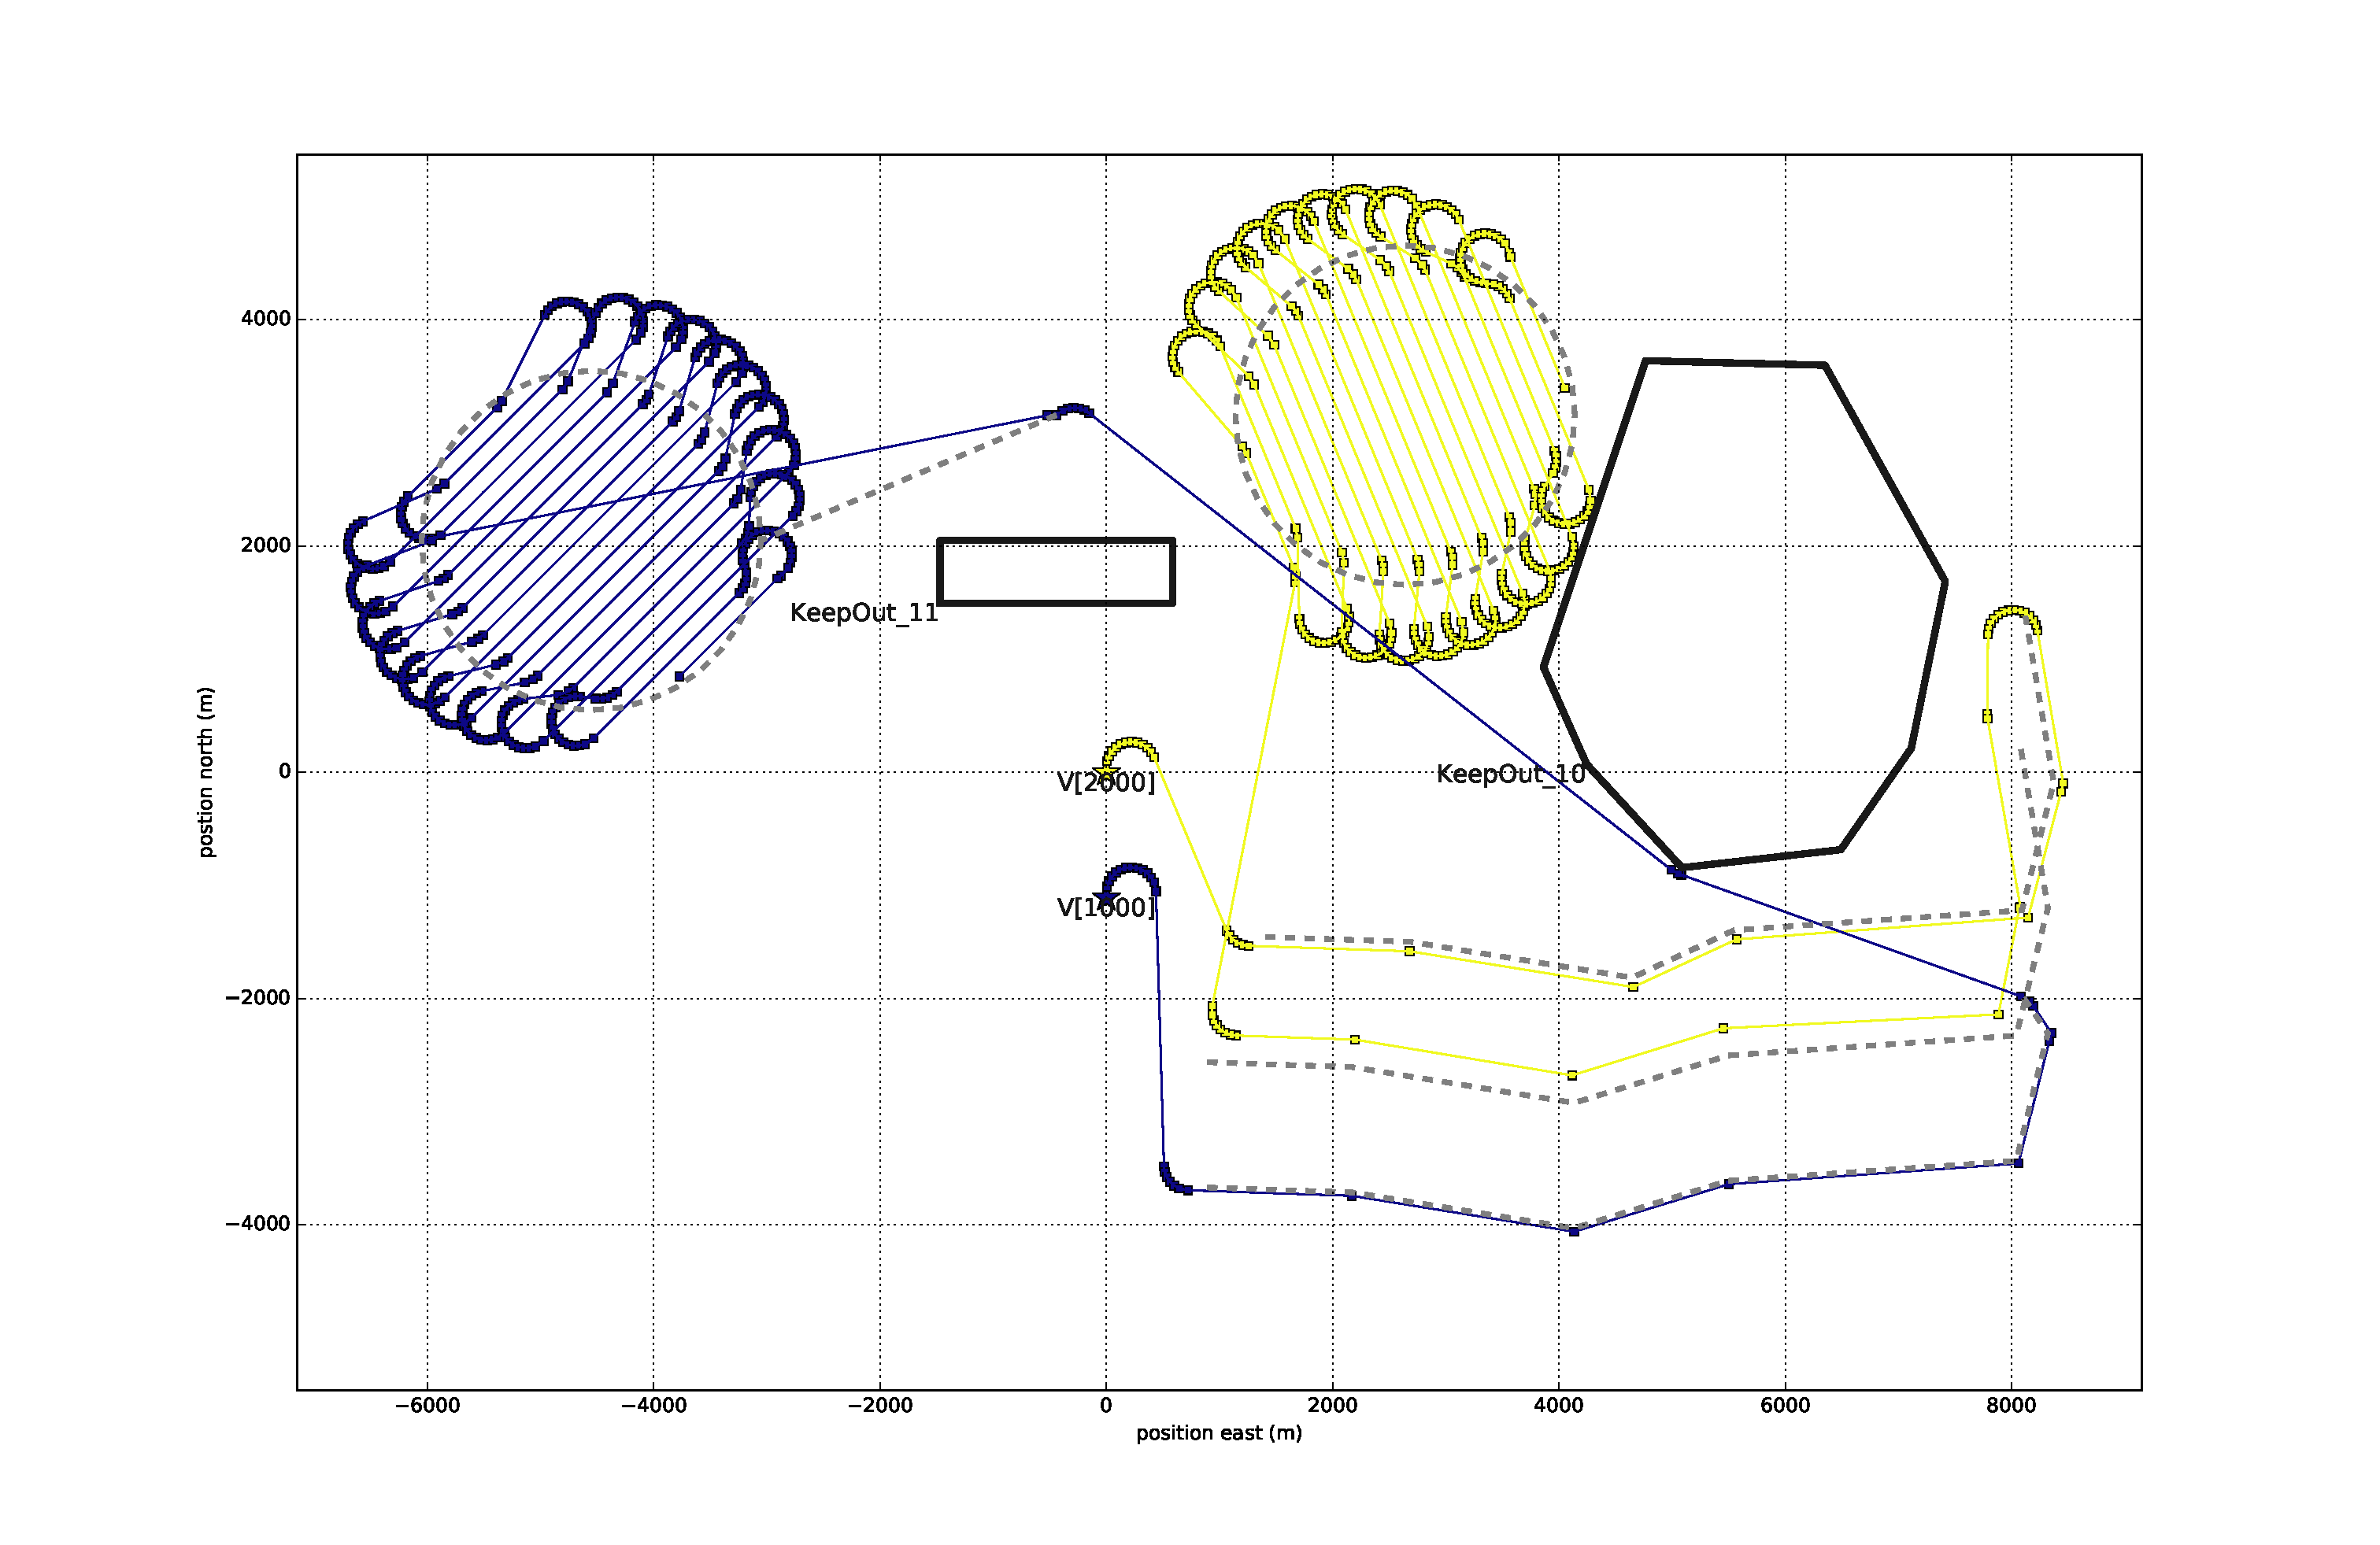
\includegraphics[width=1.65\linewidth]{\FiguresPath//02_figure_10000_all}
	\caption{Assigned UAV plans.}
	\label{fig:PlannedAssignments}
\end{marginfigure}


This example demonstrates two copies of UxAS that represent twoUAVs. They communicate with each other using a Zyre bridge, in order to synchronize the UAVs positions and headings (\textit{planning states}) that will be used to determine the trajectories and assignments for the UAVs. Since both copies of UxAS are running exactly the same trajectory/assignment algorithms, synchronizing the inputs to the algorithms will produce the same solutions on both. In this manner, each copy of UxAS generates trajectories/assignments for all UAVs and then implements the trajectories/assignment generated for itself. Both copies of UxAS are running the same algorithms as used in the fully connected case, therefore, this method of cooperation is termed "Centralized Assignment/Distributed Implementation". Figure \ref{fig:PlannedAssignments} is a plot of the resulting assigned plans for both UAVs, obtained by both copies of UxAS, 

The following LMCP messages are used to implement cooperation in this example:
\begin{description}
\item[uxas.messages.task.\textbf{AssignmentCoordinatorTask}] - task that coordinates trajectories/assignments
\item[uxas.messages.task.\textbf{CoordinatedAutomationRequest}] - sent to all UAVs, to start the coordinated assignment.
\item[uxas.messages.task.\textbf{PlanningState}] - contains the entity state that will be used for planning.
\item[uxas.messages.task.\textbf{AssignmentCoordination}] - sent to synchronize \textit{PlanningState}s with \textit{CoordinatedAutomationRequest}s
\end{description}

\begin{marginfigure}[170pt]
	\hspace{-35pt}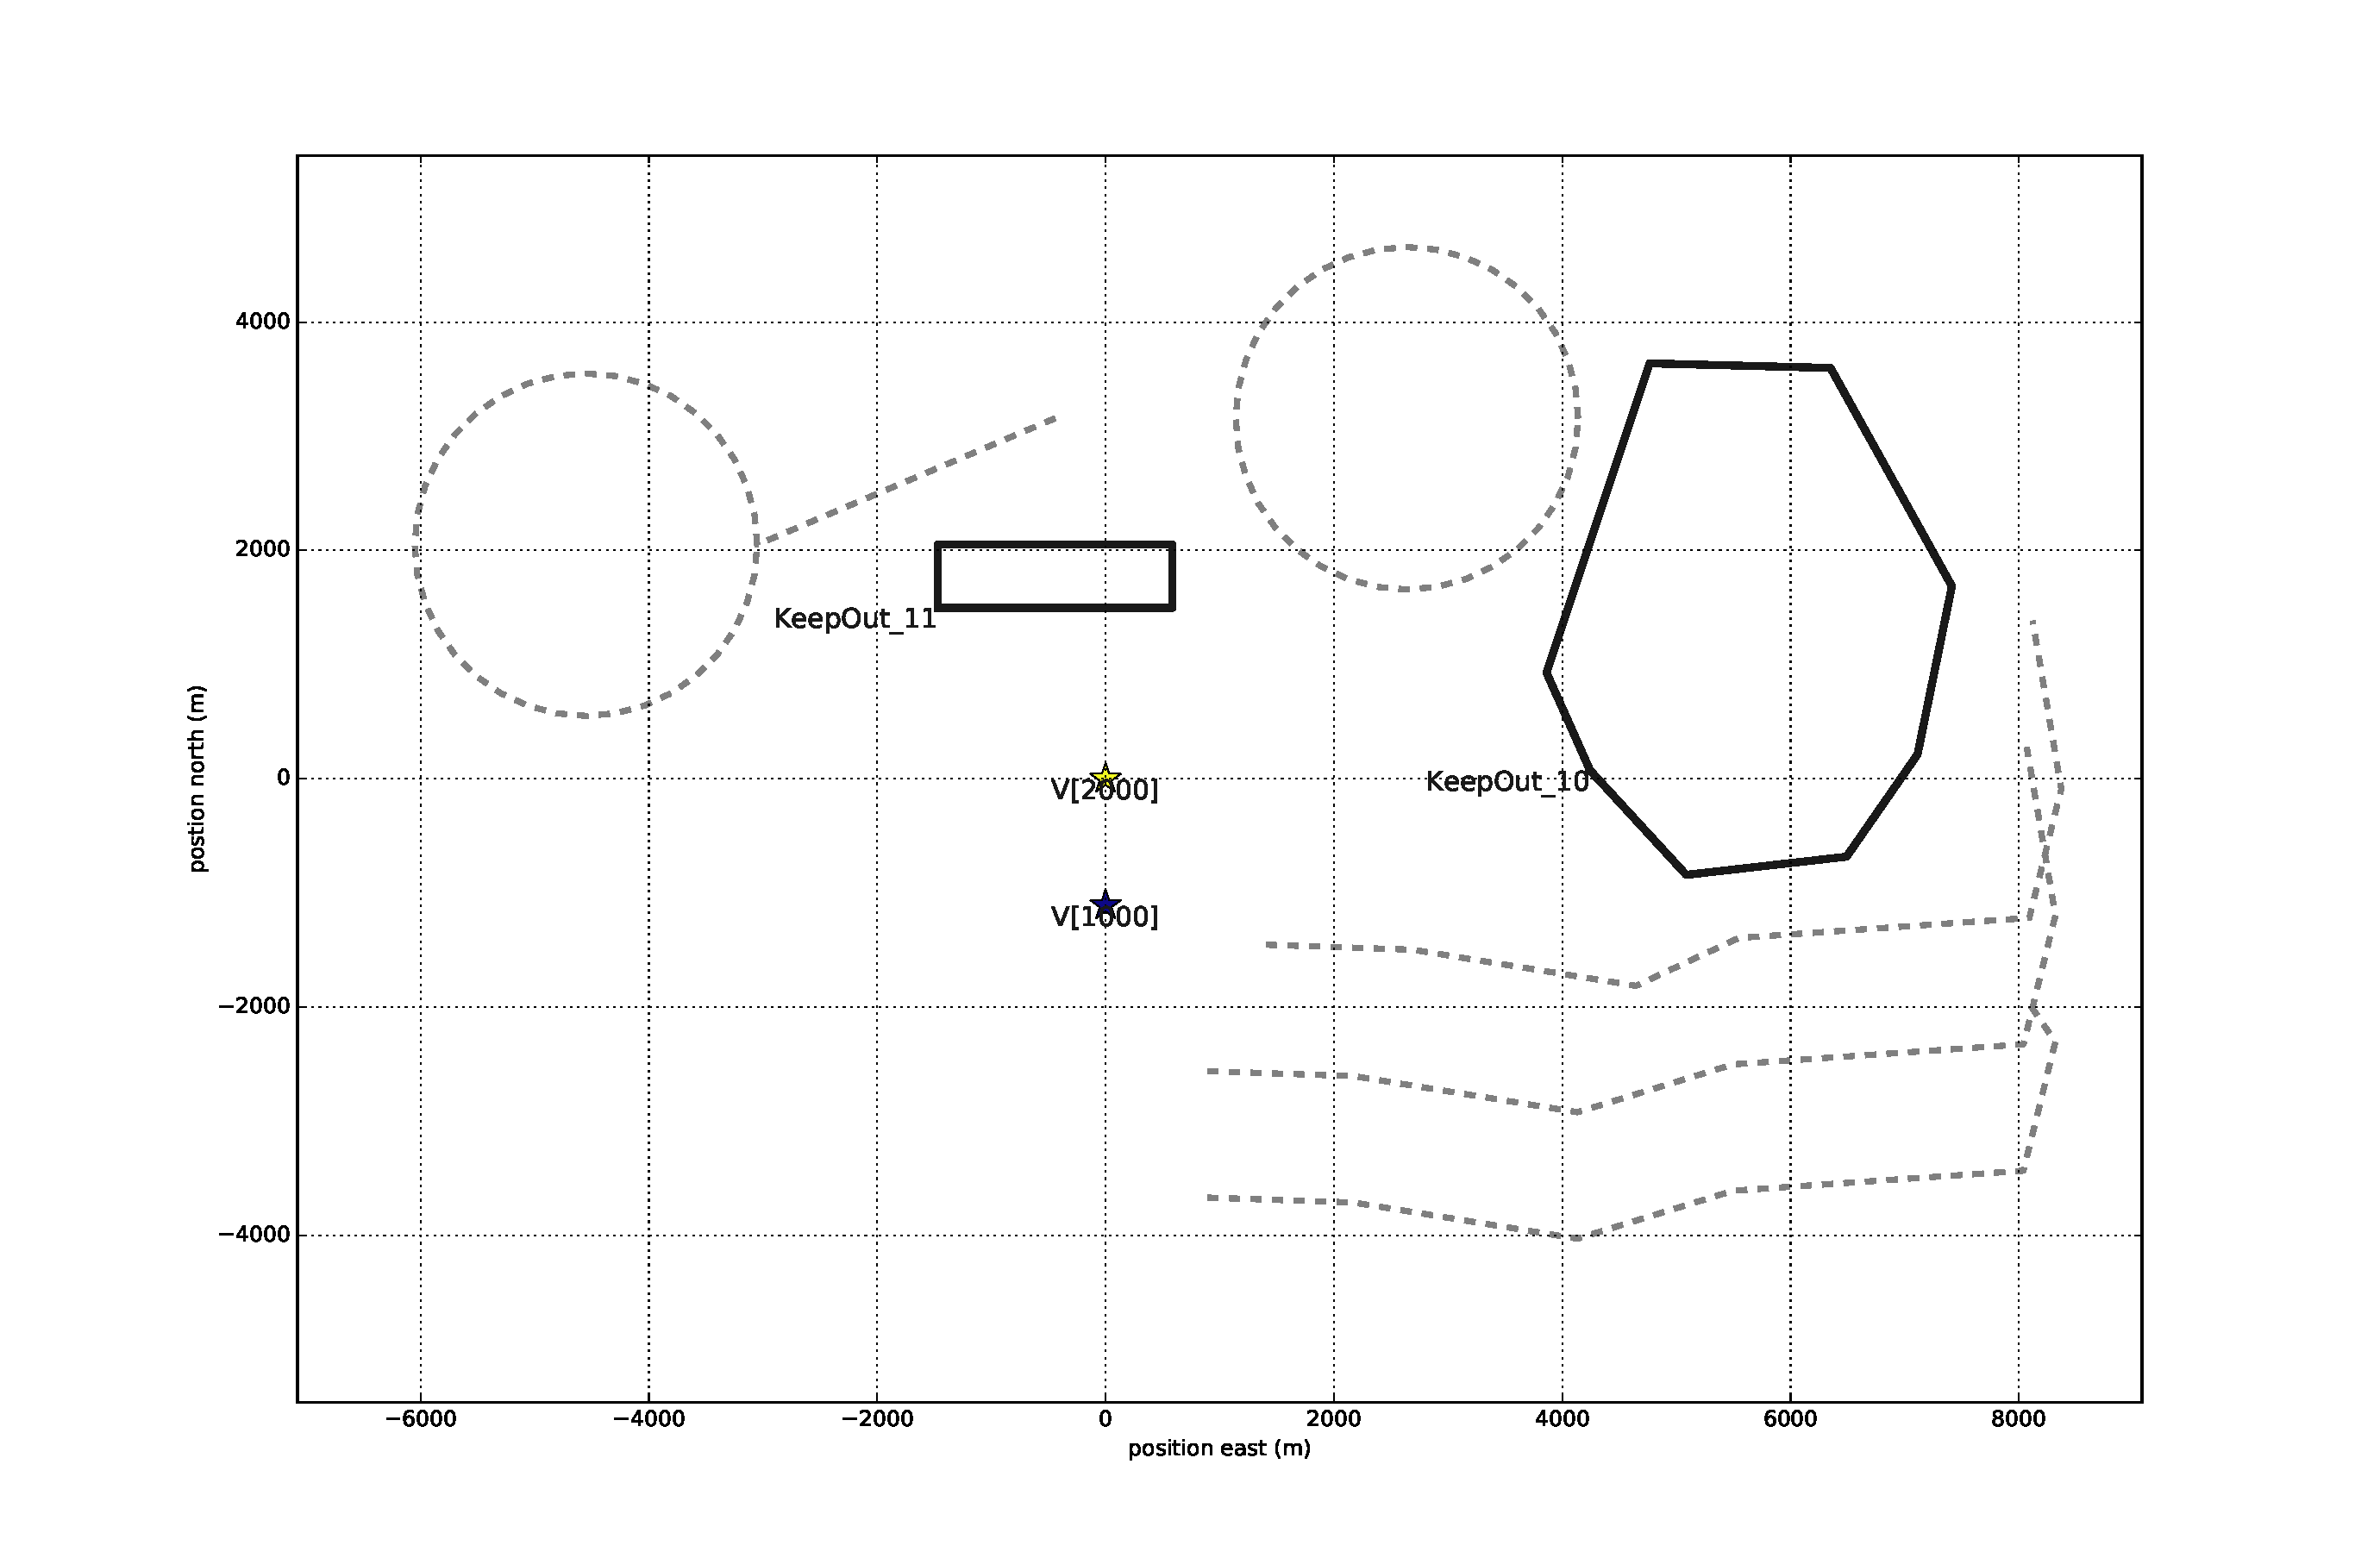
\includegraphics[width=1.65\linewidth]{\FiguresPath//01_figure_10000_tasks}
	\caption{Initial UAV positions, requested tasks, and keep-out boundaries.}
	\label{fig:InitialPositionsTasks}
\end{marginfigure}


In this example there are two UAVs, two keep-out boundaries, and five tasks, see Figure \ref{fig:InitialPositionsTasks}. In the figure UAVs 1000 and 2000 are represented by stars, keep-out boundaries 10 and 11 are polygons with solid lines, and tasks are represented by dashed lines. There are two area and three line search tasks. The example is designed to bring up two copies of UxAS, allow them to communicate to each other over a Zyre interface, and exercise the operation of the \textit{AssignmentCoordination} task and associated messages. After the copies of UxAS are initialized a "CoordinatedAutomationRequest", that specifies they coordinate with \textit{three} UAVs, is sent to each. \textit{AssignmentCoordination} tasks will exchange "\textit{AssignmentCoordination}" messages, and since there is no third UAV, wait until the specified \textit{MaximumResponseTime} to construct and send TaskAutomationRequest messages to build plans and assignments for the two UAVs to perform all five tasks. The TaskAutomationRequest messages are constructed using  \textit{AssignmentCoordination} messages, which were contained in the \textit{AssignmentCoordination} messages. The \textit{AssignmentCoordination} message contain the state that each UAV will be used for planning. Using these messages, which are synchronized on the \textit{CoordinatedAutomationRequest} ID, makes it possible to synchronize the inputs to the planning/assignment algorithms, and hence obtain a coordinated task assignment/plans for each of the vehicles. 


\begin{figure*}
	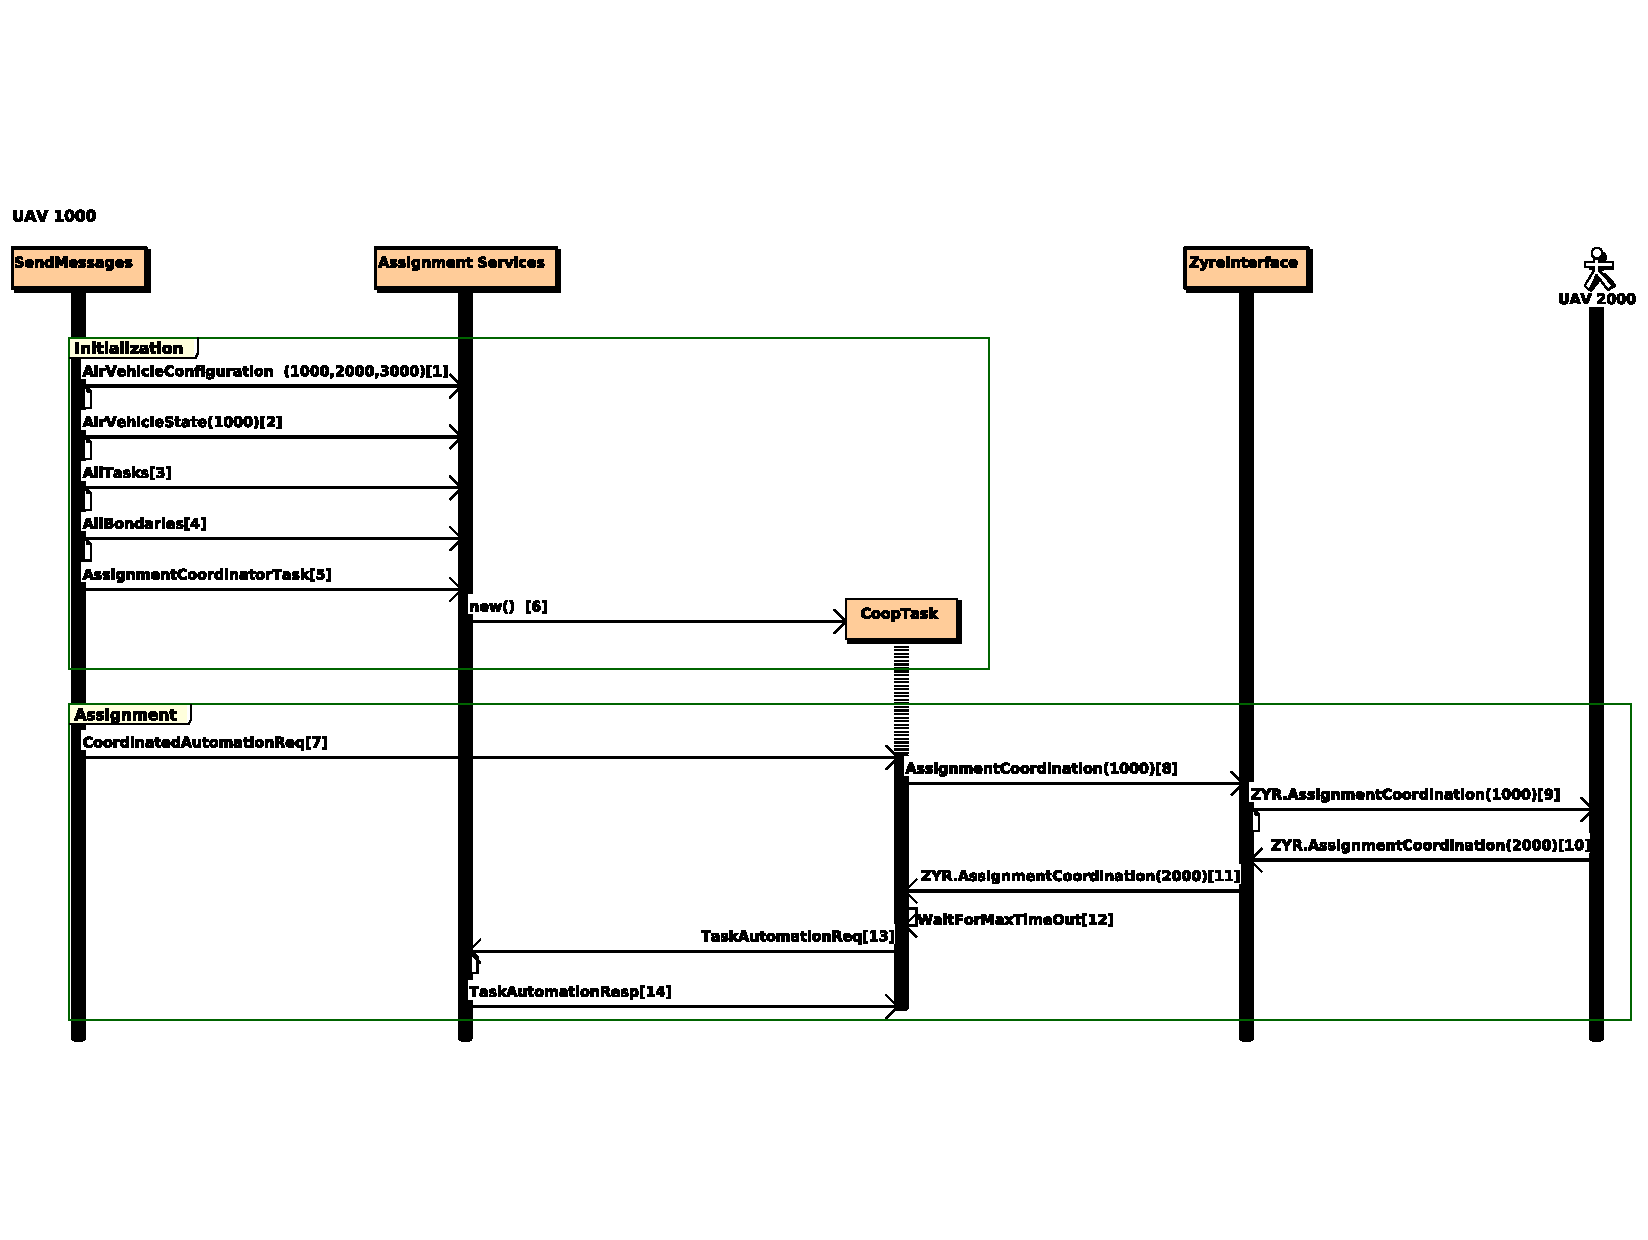
\includegraphics[width=0.8\linewidth]{\FiguresPath//DistributedCooperation_MessageFLow_Fig_all}
	\caption{Distributed cooperation example message flow.}
	\label{fig:DistributedCooperationMessageFlow}
\end{figure*}

A an message flow diagram, see Figure \ref{fig:DistributedCooperationMessageFlow}, was created to better explain the events that occur during this example. This diagram depicts the messages important to this scenario. For a more in-depth look a the message flow for assignments see the \textit{Waterway Search} example. The elements of the diagram are:

\begin{itemize}
	\item The \textbf{rectangles} across the top of the diagram, and the one in the center, represent UxAS services, which are described in the next section. 
	\item The \textbf{stick figure} labeled `UAV 2000' is the second UAV and is connected to the current UAV via a network connection. 
	\item The \textbf{horizontal lines} represent LMCP messages and the arrowheads show where messages are received. Note: messages are sent in order from top to bottom.
\end{itemize}

\newthought{UxAS Services in the Message Flow}
\begin{description}
	\item[\textit{\textbf{SendMessages}}] This service reads messages from files and then sends them out to the other UxAS services at given times. It is used to "load" initial message into UxAS, as well as, time sensitive messages such as the \textit{CoordinatedAutomationRequest}.
	\item[\textit{\textbf{Assignment Services}}] These are all the services, discussed in the Waterway example, required to plan and assign UAVs to perform tasks. 
	\item[\textit{\textbf{CoordinationTask}}] This task (service) manages/generates the messages required to coordinate the assignments. 
	\item[\textit{\textbf{Zyre Interface}}] Zyre is a ZeroMQ library that finds other entities on the local network and then makes a TCP/IP connection with them. 
	\item[\textit{\textbf{UAV 2000}}] This is the second UAV in the example. It has the same services as this one. 
\end{description}

\subsection{Message Flow Description}
The following sections describe the message flow and how it is used to implement the Distributed Cooperation Monitoring scenario. The message flow is broken into two phases: Initialization and Assignment. Each is described below. Note: this example ends after the assignments have been calculated.


\newthought{Initialization}
In this phase all the information required to calculate plans and assignments is passed into UxAS via messages.
\begin{description}
	\item[\textbf{[1] AirVehicleConfiguration(1000, 2000, 3000)}] are the set of \textbf{\textit{AirVehicleConfiguration}} Messages for UAVs 1000, 2000, and 3000. These messages provide UAV specific parameters used in planning and execution such as UAV nominal  operating speed, altitude, and maximum bank angle, as well as, sensor configurations. All UAVs considered in planning must have an AirVehicleConfiguration.
	\item[\textbf{[2] AirVehicleState(1000)}] is \textbf{\textit{AirVehicleState}} message for UAV 1000. This is the state that UAV 1000 will used to calculate plans and assignments. States for other vehicle are exchanged in the coordination process.
	\item[\textbf{[3] AllTasks} ] is the set of messages that define the tasks used in the example. This example demonstrates planning assignment for five tasks, two types of area search and two types of line search (one used twice). The messages in the set are: \textbf{AngledAreaSearchTask(ID51)}, \textbf{AreaOfInterest(ID100)}, \textbf{AreaSearchTask(ID50)}, \textbf{ImpactLineSearchTask(ID21)}, \textbf{LineOfInterest(ID101)}, \textbf{LineSearchTask(ID20)}, \textbf{LineSearchTask(ID30)}.
	\item[\textbf{[4]AllBoundaries}] is the set of messages that define the boundaries used in the example. The messages in the set define two keep-out boundaries,  \textbf{KeepOutZone(ID10)} and \textbf{KeepOutZone(ID11)}, and the operating region, \textbf{OperatingRegion(ID100)}. Note, the operating region defines which boudary ID are active.
	\item[\textbf{[5] AssignmentCoordinatorTask}] causes the \textit{TaskManager}, contained in the \textbf{AssignmentServices}, to create a new instance of the coordination task.

\end{description}
%
%
%
\newthought{Assignment}
During this phase, a special automation request is sent in which causes the assignment coordination task to manage cooperation with the other vehicles. Since there is no UAV 3000, the assignment coordination task will delay starting the assignment until expiration of the \textit{MaximumResponseTime}, which is specified in the CoordinatedAutomationRequest message.
\begin{description}
	\item[\textbf{[7] CoordinatedAutomationReq}] the \textbf{CoordinatedAutomationRequest} message contains the requested tasks and eligible UAVs to perform the tasks. Is also has a \textit{MaximumResponseTime} entry that defines the amount of time to wait for inputs from all of the eligible vehicles before initiating the assignment with a sub-set of vehicles.
	\item[\textbf{[8] AssignmentCoordination(1000)}] when a \textbf{CoordinatedAutomationRequest} message is received, the \textbf{AssignmentCoordinatorTask} calculates a state that the (local) UAV will use to complete the request. The state is put into a \textit{AssignmentCoordination} message and sent out.
	\item[\textbf{[9] AssignmentCoordination(1000)}] since the \textbf{ZyreInterface} subscribed to \textit{AssignmentCoordination} messages, it forwards the message to all connected UAVs.
	\item[\textbf{[10] AssignmentCoordination(2000)}] when the \textbf{ZyreInterface} receives a \textit{AssignmentCoordination} from a connected UAV, it is sent out to the local services.
	\item[\textbf{[11] AssignmentCoordination(2000)}] as the \textbf{AssignmentCoordinatorTask} receives \textit{AssignmentCoordination} messages, it checks to make sure they are associated with the \textit{CoordinatedAutomationRequest} and then stores them. If \textit{AssignmentCoordination} messages have been received for all of the UAVs in the \textit{CoordinatedAutomationRequest}'s \textit{EntityList}, then the \textbf{AssignmentCoordinatorTask} generates and sends a \textit{TaskAutomationRequest}.
	\item[\textbf{[12] WaitForMaxTimeOut}] since there is no UAV3000 in this example, the \textbf{AssignmentCoordinatorTask} waits for \textit{MaximumResponseTime} seconds, since receiving the \textit{CoordinatedAutomationRequest}, and then sends the request.
	\item[\textbf{[13] TaskAutomationReq}] this is the \textit{TaskAutomationRequest} message used to request planning assignment.
	\item[\textbf{[14] TaskAutomationResp}] once the plans/assignments have been calculated, they are returned in an TaskAutomationResponse message.

\end{description}


\subsection{Distributed Cooperation Example - Specifics}

This is an example of running UxAS services that communicate with each other to synchronize plannning and assignment of vehicles to tasks. The copies of UxAS exchange 'AssignmentCoordination' messages which contain the vehicle positions and headings that each vehicle will use for planning and assignment. Since the copies of UxAS are running the same assignment software, synchronizing the inputs will also synchronize the outputs. Each copy of UxAS runs the assignment algorithm for all known vehicles and implements the assignments corresponding to its own ID, this is using a "centralized" algorithm in a "decentralized" implementation.

\newthought{Files}
\begin{description}
	\item[cfgDistributedCooperation\_????.xml] - UxAS configuration file for vehicle ???? 
	\item[runUxAS\_DistributedCooperation.sh] - bash script to run the example
\end{description}
 
The '\textit{MessagesToSend}' directory contains files with xml encoded LMCP messages that are sent in to UxAS using the \textbf{MessagesToSend} service. 

\begin{description}
	\item[MessagesToSend/AirVehicleConfiguration\_V????.xml] - the air vehicle configurations for vehicles 1000, 2000, and 3000.
	\item[MessagesToSend/AirVehicleState\_V????.xml] - initial air vehicle states for vehicles  1000 and 2000.
	\item[MessagesToSend/AngledAreaSearchTask\_51.xml] - an IMPACT angled area search task.
	\item[MessagesToSend/AreaOfInterest\_100.xml] - the area that AngledAreaSearchTask\_51 will search.
	\item[MessagesToSend/AreaSearchTask\_50.xml] - a CMASI area search task.
	\item[MessagesToSend/AssignmentCoordinatorTask.xml] - the task that coordinates vehicle states before the assignment
	\item[MessagesToSend/CoordinatedAutomationRequest.xml] - the automation request used in conjunction with the AssignmentCoordinatorTask
	\item[MessagesToSend/ImpactLineSearchTask\_21.xml] - an IMPACT line search task.
	\item[MessagesToSend/KeepOutZone\_??.xml] - polygons that represent areas that the vehicle are not to enter.
	\item[MessagesToSend/LineOfInterest\_101.xml] - points of the line for ImpactLineSearchTask\_21.
	\item[MessagesToSend/LineSearchTask\_??.xml] - a CMASI line search task.
	\item[MessagesToSend/OperatingRegion\_100.xml] - the operating region, i.e. set of keep-in and keep-out tasks, to be used in the assignment.
\end{description}



\newthought{Running the Example}
\begin{enumerate}
\item open a ternimal window in the directory: \textit{examples/03\_Example\_DistributedCooperation/}
\item enter the command: \textit{./runUxAS\_DistributedCooperation.sh}
\end{enumerate}

\newthought{What Happens?}
\begin{itemize}
\item Two console windows will open, each will have UxAS running.
\end{itemize} 
\textit{FOR EACH COPY OF UxAS:}
\begin{itemize}
\item By the end of the first second, all air vehicle configurations and states, as well as all tasks and associated messages are sent in to UxAS using the 'SendMessages' service.
\item Each 'LmcpObjectNetworkZeroMqZyreBridge' will make a connection with the other copy of UxAS.
\item At two seconds an air vehicle state, corresponding to the entity ID, is sent to UxAS. This state must be sent to UxAS after the assignment coordinator task, so the task has an air vehicle state from the local vehicle.
\item At five seconds the coordinated automation request is sent in which starts the assignment process.
\item After receiving the coordinated automation request, the assignment coordinator task send out an 'AssignmentCoordination' message containg the state that the local vehicle will use for planning.
\item The 'AssignmentCoordination' is picked up by the 'LmcpObjectNetworkZeroMqZyreBridge' and sent to the other running copy of UxAS
\item The assignment coordinator recieves the 'AssignmentCoordination' message from the UxAS and checks to see if its time to send in a TaskAutomationRequest. The 'CoordinatedAutomationRequest' specifies three vehicle IDs and since the the third vehicle is not present, the assignment coordinator must wait untile the specified has passed, 10 seconds from recipt of the request, to sent out the 'TaskAutomationRequest'.
\item Once the timer has expired, a 'TaskAutomationRequest' specifing two vheicles is sent out. This causes the UxAS services to calculate assignments for both vehicle.
\item The resulting assignment can be plotted using the python scripts located in the sub-directory of:
\begin{docspec}
03\_Example\_DistributedCooperation/UAV\_1000/datawork/AutomationDiagramDataService/
\end{docspec}
\end{itemize} 

\newthought{Things to Try}
\begin{itemize}
\item Edit the automation request,
\begin{docspec}
\textit{03\_Example\_DistributedCooperation/MessagesToSend/CoordinatedAutomationRequest.xml}
\end{docspec}
and comment out, or remove the entry '\textit{<int64>3000</int64>}' in the '\textit{EntityList}'. Rerun the example. Since it will have '\textit{AssignmentCoordination}' for all of the requested vehicle, the assignment coordinator will not have to wait until the end of the '\textit{MaximumResponseTime}' to start the assignment process.
\end{itemize} 
